\documentclass[12pt,fleqn]{article}

\usepackage[utf8]{inputenc}
\usepackage[T2A]{fontenc}
\usepackage{amssymb,amsmath,mathrsfs,amsthm}
\usepackage[russian]{babel}
\usepackage{graphicx}
\usepackage[footnotesize]{caption2}
\usepackage{indentfirst}
\usepackage{amsfonts}
\usepackage{algorithm}
\usepackage{algpseudocode}
\usepackage{algorithmicx}
\usepackage{enumitem}


\usepackage{comment}
%\usepackage[ruled,section]{algorithm}
%\usepackage[noend]{algorithmic}
%\usepackage[all]{xy}

% Параметры страницы
\textheight=24cm
\textwidth=16cm
\oddsidemargin=5mm
\evensidemargin=-5mm
\marginparwidth=36pt
\topmargin=-1cm
\footnotesep=3ex
%\flushbottom
\raggedbottom
\tolerance 3000
% подавить эффект "висячих стpок"
\clubpenalty=10000
\widowpenalty=10000
\renewcommand{\baselinestretch}{1.1}
\renewcommand{\baselinestretch}{1.5} %для печати с большим интервалом

\setlist[enumerate,itemize]{leftmargin=0pt,itemindent=2.7em}

\begin{document}

\begin{titlepage}
\begin{center}
    Московский государственный университет имени М. В. Ломоносова

    \bigskip
    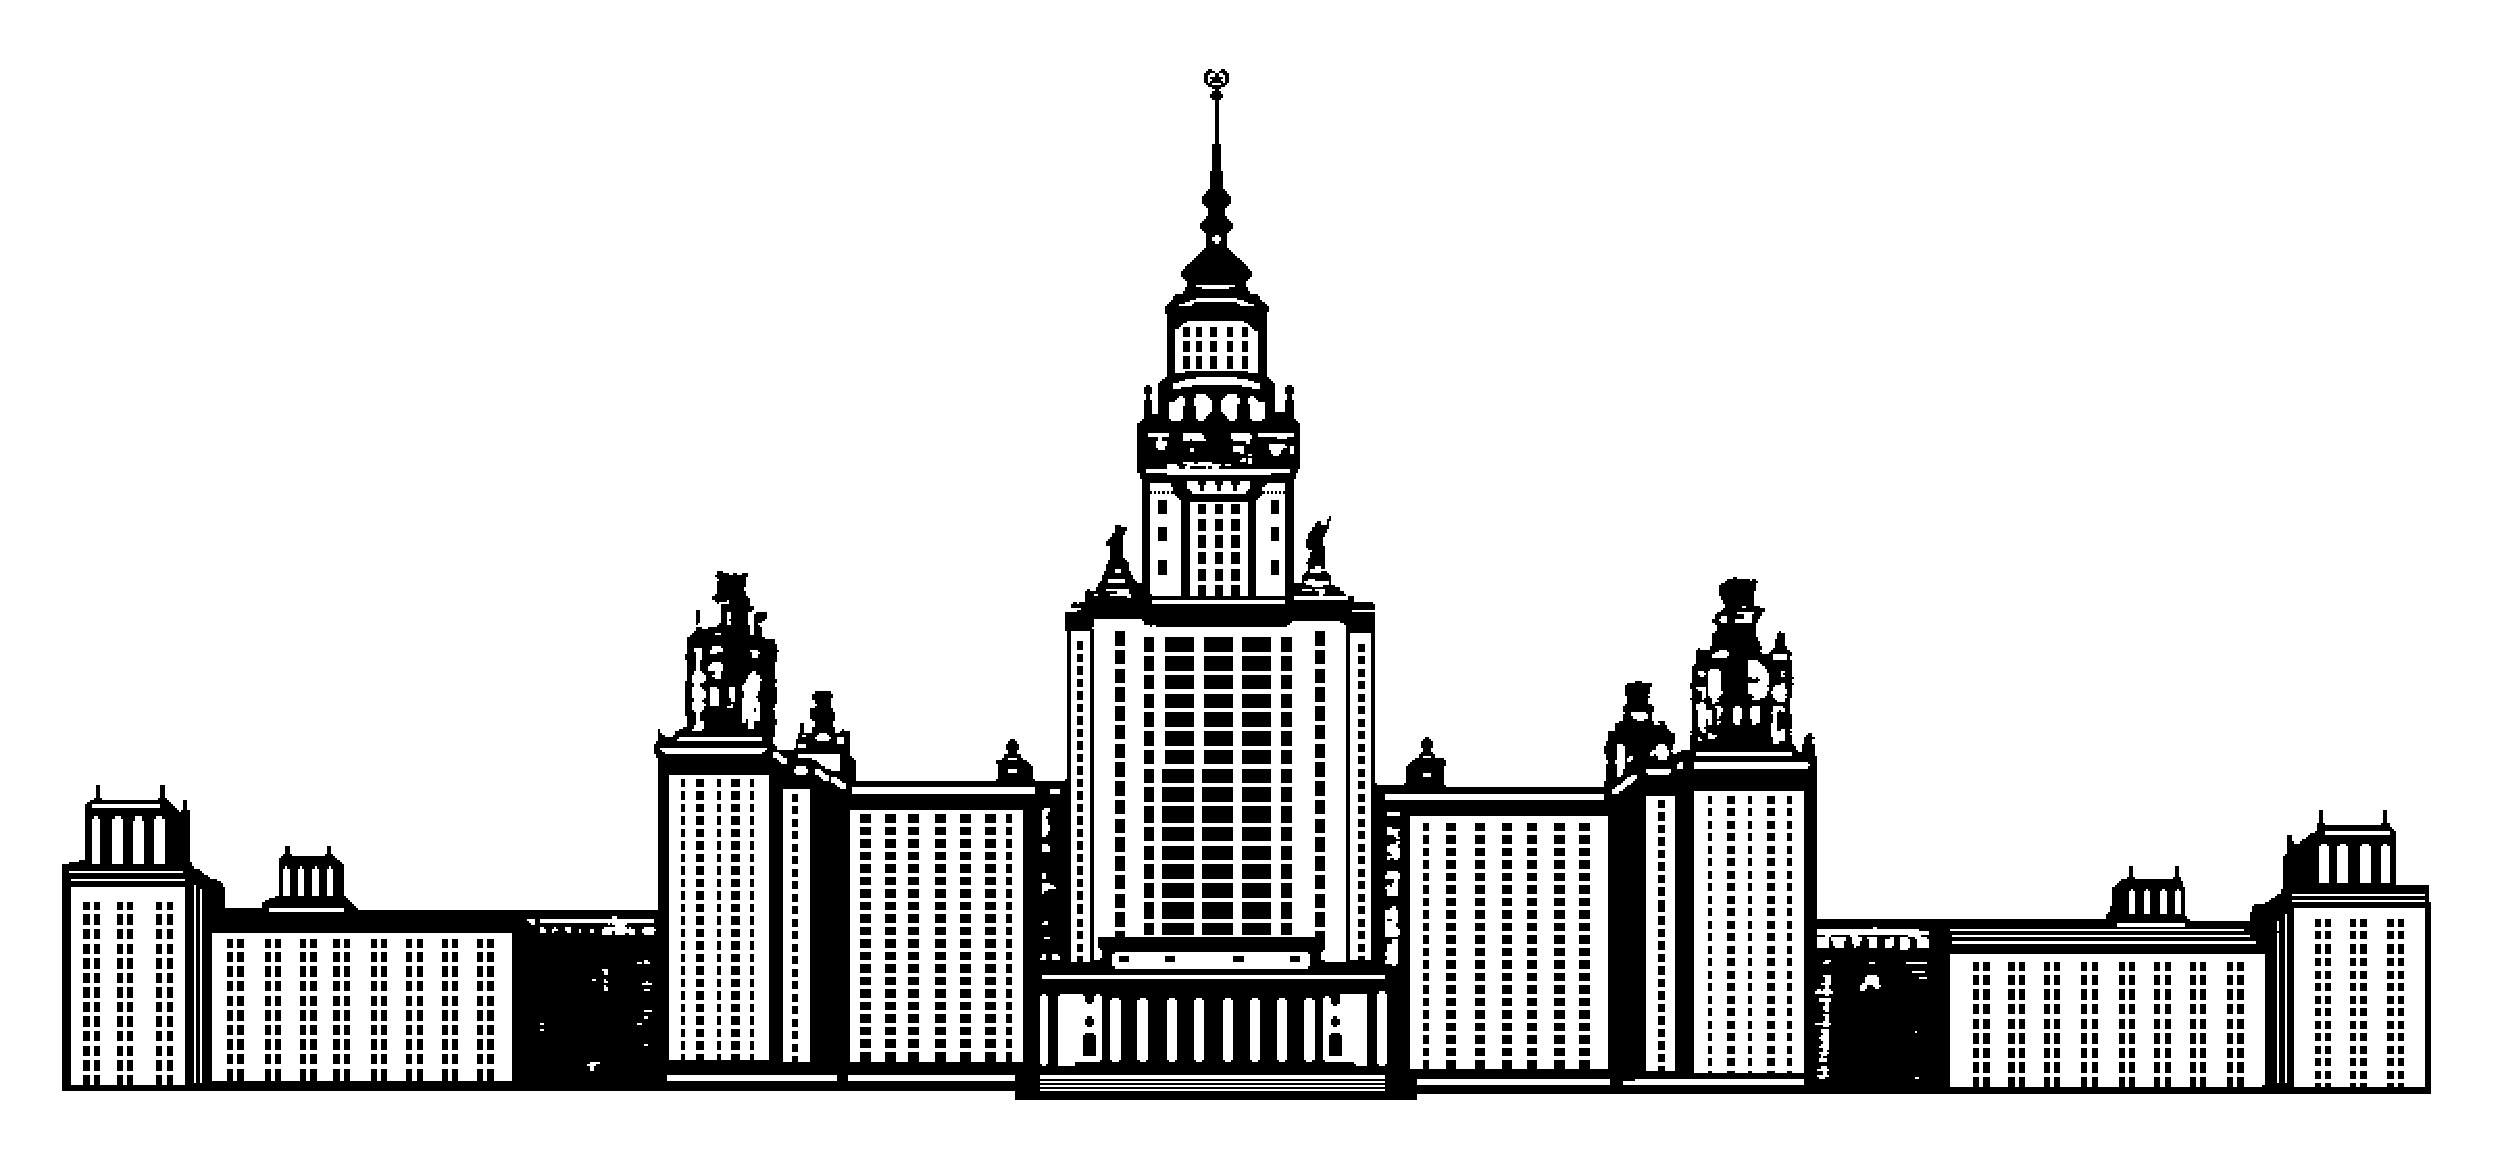
\includegraphics[width=50mm]{msu.eps}

    \bigskip
    Факультет Вычислительной Математики и Кибернетики\\
    Кафедра Математических Методов Прогнозирования\\[10mm]

    \textsf{\large\bfseries
        КУРСОВАЯ РАБОТА СТУДЕНТА 317 ГРУППЫ\\[10mm]
        <<Задача кластеризации зашумлённых данных с неоднородной плотностью >>
    }\\[10mm]

    \begin{flushright}
        \parbox{0.5\textwidth}{
            Выполнил:\\
            студент 3 курса 317 группы\\
            \emph{Демин Георгий Александрович}\\[5mm]
            Научный руководитель:\\
            д.ф-м.н., профессор РАН\\
            \emph{Дьяконов Александр Геннадьевич}
        }
    \end{flushright}

    %\newenvironment{comment}{}{}

\begin{comment}
        \begin{tabular}{p{0.45\textwidth}p{0.45\textwidth}}
            Заведующий кафедрой\newline
            Математических Методов\newline
            Прогнозирования, академик РАН
            &
            ~\newline~\newline
            \hfill\hbox to 0.45\textwidth{\hrulefill~Ю. И. Журавлёв}
        \\[20mm]
            К защите допускаю\newline
            \hbox to 0.4\textwidth{<<\hbox to 12mm{\hrulefill}>> \hrulefill~2019 г.}
            &
            К защите рекомендую\newline
            \hbox to 0.45\textwidth{<<\hbox to 12mm{\hrulefill}>> \hrulefill~2019 г.}
        \end{tabular}
\end{comment}

    \vspace{\fill}
    Москва, 2019
\end{center}
\end{titlepage}

\newpage
\renewcommand{\contentsname}{Содержание}
\tableofcontents

\newpage
\begin{abstract}
    В работе представлен подход к кластеризации зашумлённых данных с неоднородной плотностью, при наличии некоторой априорной информации о распределении кластеров.

   Предложенный подход сравнивается с классическими методами кластеризации на примере задачи выделения скоплений галактик по каталогу SDSS.


\end{abstract}

\newpage
\section{Введение}
Задача кластеризации в машинном обучение - типичная задача обучения без учителя: есть некоторые показатели, которые сигнализирует о том, хорошо решена задача или нет, но точной информации нет. Обычно эта задача является промежуточным этапом построения модели в машинном обучении. Она может использоваться для добавления к объектам признаков, уменьшения объёма данных путём объеденения объектов, попавших в один кластер. Также целью может служить - понимание структуры данных и их распределения. Более подробно задача кластеризации описана в разделе ''постановка задачи''.

В данной работе рассматривается задача кластеризация на данных, о которых известно, что большая их часть в кластеры не входит и является шумом. Кроме того, известно, что данные неоднородны и их плотность варируется. Предполагается также, что имеется некоторая априорная информация о распределении кластеров. Такая задача может возникнуть при распознавании образов, анализе биологических или физических систем.

Предлагается алгоритм, основанный на DBSCAN, учитывающий некоторые априорные представления о данных и адаптирующийся, способный настраиваться на варьирующуюся плотность. Алгоритм используется для решения задачи кластеризации галактик из каталога SDSS. Результаты его работы сравниваются с результатами, полученными с помощью ''классических'' алгоритмов (mean shift, классический DBSCAN)

Опишем более подробно задачу кластеризации и её типы.

\section{Постановка задачи}\label{problem}

\subsection{Задача кластеризации в машинном обучении}

Задача кластеризации в машинном обучении - это задача разбиения выборки объетов на некоторые множества, называющиеся кластерами, при этом одному множеству должны принадлежать в некотором роде похожие объекты, а объекты из разных кластеров - существенно отличаться. Входными данными для задачи кластеризации могут быть как объекты и их признаковое описание, так и матрица расстояний (или схожести) между объектами.

Особенностью этой задачи является то, что её решение принципиально неоднозначно: нет точной постановки задачи, существует много критериев качества кластеризации, результат решения задачи сильно зависит от выбранной метрики (или схожести близости), качество кластеризации определяется во многом спецификой задачи (один и тот же результат может восприниматься как хороший или плохой в зависимости от того, для чего именно мы кластеризуем данные).


Для решения задачи могут применяться различные алгоритмы в зависимости от того, какой структура кластеров ожидается. На основании этого задачу кластеризации разделяют на (см. \cite{cluster_class}):
\begin{itemize}
\item \textbf{Иерархическая} или \textbf{плоская}. Под иерархической  структурой кластеров понимается такое их устройство, что некоторые мелкие кластеры могут быть объеденены в более крупные, которые в свою очередь также могут быть объеденены в ещё б\'{о}льшие. Плоская кластеризация подразумевает, что некоторое множество выделенных кластеров не может само образовывать боллее большой кластер.
\item \textbf{Исключающая}, \textbf{перекрывающая} или \textbf{нечёткая}. Исключающая кластеризация означает, что объект может быть отнесён только к одному классу, перекрывающая - к нескольким. Нечёткая кластеризация является частным случаем перекрывающей и для каждого объекта определяет вероятность вхождения в каждый кластер (другое её название - \textbf{вероятностная}).
\item \textbf{Полная} или \textbf{частичная}. При полной кластеризации каждый объект обязательно относится к кому-либо кластеру, а при частичной объект может являться шумом или выбросом и не должен принадлежать кластеру.
\item \textbf{Прототипная}, \textbf{графовая} или \textbf{плотностная}. При прототипной кластеризации кластер определяется как множество объектов, похожих на некий прототип. Графовая модель --- модель, при которой данные представлены в виде графа и кластером будет являться некое подмножество вершин, которые имеют большое количесвто связей или образуют отдельную связную компоненту. Плотностная кластеризация же означает, что кластером будут считаться объекты, плотность (при каком-то заданном распределении) которых больше средней плотности всей выборки.
\end{itemize}

В данной работе мы будем решать плоскую исключающую плотностную задачу кластеризации. Кроме того, ожидаем, что большая часть данных относится к шуму

\subsection{Формальная постановка задачи}
Приведём формальную постановку задачи: имеется $X \in \mathbb {R}^{N \times D}$ -  матрица объекты-признаки, $D \ll N$. $S = \{0, 1, ..., K \}$ - множество номеров кластеров, K (число кастеров) априорно неизвестно. Требуется найти отображение $y(x): X \rightarrow Y$, где $Y_i \in S$ и является номером кластера, которому принадлежит $X_i$.
 $y(x_0) = 0$ означает то, что объект $x_0$ является шумовым и не принадлежит ни одному кластеру. Кроме того, мы предполагаем, что
\begin{itemize}
\item Кластеризация производится на основе плотности.

\item Число объектов, не относящихся ни к какому кластеру велико
\begin{equation}\label{more_noize}
         \frac{|\{x|y(x)=0\}|}{|X|} \geqslant 0.5.
      \end{equation}

\item Имеется некое априорное представление о структуре кластеров
\begin{equation}\label{features}
         \exists  F_i(Y, K) \approx C_i, i = \overline{1, m}.
      \end{equation}
\end{itemize}

\section{Обзор существующих решений}

\subsection{Сдвиг среднего значения (mean shift)}
Сдвиг среднего значения является алгоритмом поиска локальных максимумов плотности вероятности, задаваемой дискретной выборкой объектов. Идея заключается в том, что на каждой итерации каждая точка сдвигается в направлении наибольшей плотности. 
$K(t) = K(||t||^2)$ - неотрицательная невозрастающая функция, называемая ядром, вместо $t$ обычно рассматривается разность между двумя точками. Это функция выражает то, что объекты, находящиеся ближе к рассматриваемому объекту влияют на него сильнее, чем далёкие.
Обычно также полагают, что при $t > h$ (h - некий порог) $K(t)=0$, то есть мы не учитываем влияние объектов, находящихся вне небольшой окрестности. Также обычно использется так называемое Гаусово ядро:
\begin{equation*}
K(t) =
 \begin{cases}
   e^{-\frac{t}{2h^2}} &  t < h\\
   0 & t \geq h
 \end{cases}
\end{equation*}

Итак на каждом шаге для каждого объекта $x$ вычисляется 
\begin{equation*}
m(x) = \frac{\sum_{x_i \in G(x)}^{}K(x-x_i)x_i}{\sum_{x_i \in G(x)}^{}K(x-x_i)}.
\end{equation*}
Это новые координаты объекта $x$ (за $G(x)$ обозначена окрестность, в которой $K(x-x_i) \neq 0$, таким образом текущий объект сдвигается в направлении увеличения плотности. Данный итерационный процесс продолжается, пока $||x - m(x)||^2 > \epsilon $. После завершения все объекты, находящиеся очень близко (  $||x_i - x_j||^2 < \delta $) назначаются в один кластер.

Этот алгоритм имеет ряд преимуществ:  произвольность в выборе ядерная функции позволяет учитывать некоторые априорные знания о кластерах, он имеет единственный настраиваемый параметр - $h$, также изначально не требуется указывать число кластеров. Недостатком является то, что выбор $h$ нетривиален и от него серьёзно зависит результат кластеризации, также иногда требуется использовать настраивающуюся ширину окна в зависимости от конкретных данных.


\subsection {DBSCAN}
В основе алгоритма DBSCAN лежит другая идея: в окрестности точки, лежащей в кластере будет лежать много точек, тоже лежащих в кластере.
Должны быть заданы 2 параметра: $minPts$ - минимальное число точек в окрестности данной такое, чтобы данная точка входила в кластер и $eps$ - радиус окрестности.

Основной точкой называется точка, в окрестности, которой содержится больше, чем $minPts$ точек. Граничная точка - не основная точка, но лежащая в окрестности какой-то основной. Шумовые точки - все остальные точки. Алгоритм заключается в том, что для каждой точки мы определяем её тип, выкидываем шумовые и объединяем все основные и граничные точки, связанные между собой в кластер. Таким образом мы получаем непересекающееся множество кластеров.

Основное преимущество DBSCAN - выделение кластеров произволной формы, а также быстрое выполнение (при грамотной организации структур данных алгоритм работает за время $\mathcal{O}(n\log{}n)$). Недостатками является то, что нужно подбирать 2 параметра (в данных с неоднородной плотностью это особенно трудно сделать), качество алгоритма серьёзно зависит от измерения расстояния.


Далее рассмотрим некоторые модификации алгоритма DBSCAN, на которые будет существенно опираться предложенный ниже подход.

\subsubsection{VDBSCAN}
Для набора данных с варирующейся плотностью в статье \cite{VDBSCAN} был предложен следующий подход: запустить алгоритм DBSCAN несколько раз с разными значениями радиуса. При каждой последующей итерации исключать точки, кластеризованные на предыдущей, - таким образом могут быть обнаружены кластеры с различной плотностью. В статье \cite{AutoVDBSCAN} описывается способ для определения параметров k и eps. Предлагается посчитать среднее расстояние между точками в датасете, затем для каждой точки посчитать какой по номеру ближайший сосед отстоит от неё на это расстояние и взять в качестве
k - самый частый номер среди всех точек. Далее для каждой точки находится расстояние от неё до k-го ближайшего соседа, строится гистограмма таких расстояний и резкие скачки на ней будут считаться кандидатами на eps.
У этого подхода есть несколько недостатков: во-первых, в нём слабо учитываются априорные знания о данных (только то, что они имеют неоднородную плотность), во-вторых, он не подходит для датасета с большим количеством шума, так как гистограмма расстояний до k-го ближайшего соседа не позволит определить значения eps (она будет слишком гладкой из-за расстония до шумовых точек)

\subsubsection{Дифференциальная эволюция для подбора параметров DBSCAN}
Дифференциальная эволюция --- это метод стохастической оптимизации(см. \cite{dif_evol}). Его идея в том, что генерируется некоторое множество алгоритмов с разными параметрами - популяции (при этом используется один и тот же алгоритм и изменяются лишь его параметры), для каждого алгоритма вычисляется функция потерь. Алгоритмы, значения функций потерь которых, оказались низкими, скрещиваются и получившийся алгоритм получает параметры, близкие к параметрам его предков. неудачные же алгоритмы с некоторой вероятностью мутируют, изменяя свои параметры. Несомненное преимущество этого метода в том, что он подходит для оптимизации вообще любых алгоритмов (однако вопрос о сходимости остаётся открытым). В \cite{BDE-DBSCAN} авторы используют этот подход, чтобы подобрать k и eps для алгоритма DBSCAN. Это довольно удачный способ для нашей постановки задачи, так как все \ref{features} могут быть учтены в функции потерь и параметры будут подобраны строго автоматически. Однако в этом методе тяжело учесть то, что данные неоднородные.

Для алгоритма DBSCAN есть множество усовершенствований, однако каждое из них имеет собственные недостатки, не позволяющие решить исследуемую задачу достаточно хорошо. Ниже будет представлен метод, опирающийся на приведённые выше модификации  DBSCAN.

\section{Предлагаемый подход}
В основе предлагаемого подхода лежит одна простая идея: для областей с разной плотностью нужно использовать алгоритм с разными параметрами.
\begin{enumerate}
    \item Разбиваем признаковое пространство на подпространства с более-менее однородным распределением объектов(для этого можно построить распределение признаков и делить некоторые из них.
    \item  Определяем некоторую функцию потерь, зависящую от (\ref{features}), с помощью неё на каждом подпространстве находим параметры алгоритма DBSCAN, при этом слишком маленькие по размеру выделенные кластеры относим к шуму, чтобы учесть (\ref{more_noize}).
    \item Выделяем из подпространств зоны, на которых работа алгоритма нас не устраивает (это можно сделать на основе функции потерь или отдельных условий \ref{features}) И повторяем шаги независимо в каждой такой зоне.
\end{enumerate}

\newpage

\begin{algorithm}
\caption{DBSAN for variety density}\label{alg:Example}
\begin{algorithmic}
\Function{TuneOnSubareas}{$subareas$}

\For{$X_i \in subareas$}
    \State eps, k  $\gets$ \Call{OptimizeDBSCAN}{$X_i$, LossFunc1}
    \State $labels \gets labels ~ \cup$ \Call{DBSCAN}{$X_i$, eps, k}
\EndFor

\State \Return $labels$
\EndFunction

\State $subareas \gets$ \Call{GetSubareas}{$X$}
\State $labels \gets \{\}$
\State $labels\_first\_step \gets \Call{TuneOnSubareas}{subareas}$
\State $bad\_labels \gets$ \Call{FindBadLabels}{labels, LossFunc2}
\State $bad\_subareas \gets subareas[ bad\_labels ]$
\State $labels\_first\_step \gets labels\_first\_step~\backslash~bad\_labels$
\State $labels\_result \gets labels ~ \cup$ \Call{TuneOnSubareas}{$bad\_subareas$}
\State \Return $labels\_result$

\end{algorithmic}
\end{algorithm}

Функция GetSubareas  неким образом разбивает $X$ на подвыборки
LossFunc1, LossFunc2 неким образом отражают апрорную информацию и штрафуют за нарушение (\ref{features})
OptimizeDBSCAN подбирает параметры для алгоритма DBSCAN на подвыборке, используя дифференциальную эволюцию, a DBSCAN применяет алгоритм с подобранными параметрами. Наконец, FindBadLabels определяет какие данные были кластеризованы плохо (в следствие различия в плотности или чего-то другого).

Далее покажем, как все можно составить функции потерь, используя априорные знания на реальных данных.

\section{Набор данных. Каталог SDSS}

Продемонстрируем предлагаемый алгоритм на задаче выделения галактик по каталогу SDSS(\cite{SDSS}). Этот каталог содержит сферические координаты и некоторые физические величины более чем 3 миллионах галактик, наблюдаемых в северном полушарии Земли. \textbf{Расстояние} до галактики определяется с помощью измерения красного смещения электромагнитных волн, излучаемых ею, близкими считаются галактики, имеющие красное смещение меньше 0.3 (всюду далее под расстоянием до галактики мы будем подразумевать красное смещение этой галактики). Особенностью этих данных является то, что для галактик сильно удалённых от Земли погрешность вычислений координат достигает больших значений - это не позволяет их анализировать. \textbf{Кластером} (скоплением или глобуларом) называется набор галактик, расположенных близко друг к другу (более точного определения дать не удаётся, так как объективные характеристики, по которым можно было бы определить что явлется кластером, а что нет, пока в астрофизике не определены). Считается также, что галактика принадлежит либо принадлежит только одному кластеру, либо не принадлежит никакому (таких галактик большинство и мы будем называть их шумовыми).
Ожидается, что кластеры будут сферической или элипсовидной формы

\section{Эксперименты}
\subsection{Априорные представления и их формализация}

В качестве априорных представлений о струтуре кластеров мы возьмём результаты работы Дж.~Эйбелла \cite{Abell}. Американский астроном вручную проанализировал фотопластины северной части звёздного неба и выделил 2712 кластеров. Так как это было сделано по фотометрическим данным, нельзя сказать, что координаты выделенных кластеров точны. Мы будем использовать 2 факта из работы физика: число кластеров приближённо известно и равно 1570\footnote{Каталог SDSS покрывает не все области видимого неба, поэтому ожидается меньшее число кластеров}, характерный размер кластера примерно 125-175 галактик.
Обозначим за $N(k)$ количество объектов в кластере с номером $k$, и фоормализуем априорную информацию таким образом
\begin{equation}\label{F_num_clusters}
  F_1(Y, K) = F_1(|Y|, K) = |K -  1572\cdot \frac{|Y|}{|X|}| - 50  \leq 0
\end{equation}
\begin{equation}\label{F_num_in1cluster}
  F_2(Y, K) =  F_2(N(1), \dots, N(K), K) = \frac{1}{K} \sum_{k=1}^K \left( | N(k) -150 | - 50 \right)  \leq 0
\end{equation}

Неравенства (\ref{F_num_clusters}) и (\ref{F_num_in1cluster}) не стоит понимать строго: это лишь наши предположения, они могут нарушаться. Исходя их этого построим функцию потерь для оптимизации DBSCAN. Будем штрафовать алгоритм, если он выделяет не то количество кластеров, которое нам нужно и если в кластерах оказывается намного больше или меньше галактик, чем предполагалось. Для этого хорошо подходит квадратичная функция.
$$f_1(K) = a_1K^2 + b_1K + c_1$$
$$f_2(N(i)) = a_2N(i)^2 + b_2N(i) + c_2$$

Коэффициенты определим из условий
\begin{equation}\label{system_num_cl}
 \begin{cases}
   f_1|_{K=1572 \cdot \frac{|Y|}{|X|}} = 0
   \\
   f_1|_{K=1572 \cdot \frac{|Y|}{|X|} + 50} = 1
   \\
   f_1|_{K=1572 \cdot \frac{|Y|}{|X|} - 50} = 2.5
 \end{cases}
\end{equation}

\begin{equation}\label{system_num_in1cl}
 \begin{cases}
   f_2|_{N(i)=150} = 0
   \\
   f_2|_{N(i)=100} = 2
   \\
   f_2|_{N(i)=200} = 1
 \end{cases}
\end{equation}


Ясно, что получается 2 СЛАУ, коэффициенты которых легко находятся. Заметим, что мы полагаем квадратичную функцию равной нулю в точках с ожидаемым значением, и накладываем некоторый штраф в точках, удалённых на 50 от ожидаемого значения --- этот отступ, как и штрафы, вообще говоря, можно выбирать по-другому. Введём, наконец, функции потерь.

LossFunc2 $=\mathfrak{L}_2(Y, K) = \underset{i}{arg}\{N(i)>T\}$

LossFunc1 $= \mathfrak{L}_1(Y, K) = f_1(K) + \frac{1}{K} \sum_{i \in S\backslash \mathfrak{L}_2(Y, K)}^{}f_2(N(i))$

Эти функции с одной стороны учитывают априорные условия и с другой учитывают то, что данные имеют неоднородною плотность. Действительно, мы настраиваем DBSCAN таким образом, чтобы кластеры получались характерного небольшого размера, но если какой-то кластер получается слишком большим, мы его не учитываем и не штрафуем за него, вместо этого считаем, что распределение объектов, входящих в него имеет большую плотность и требуется для них подобрать другие параметры. Заметим, что мы никак не штрафуем количество галактик, которые определяются как шумовые, так как ограничения на количество объектов в каждом кластере и на количество самих кластеров по сути учитывают это.


\subsection{Применённые алгоритмы}

Мы будем сравнивать результаты работы 3 основных алгоритмов
\begin{itemize}
    \item
        Mean shift
    \item
        Mini Batch K-means (спецификация K- means, которая для пересчёта центра кластера на каждой итерации использует не все объекты, принадлежащие ему, а лишь некоторую их подвыборку, что очень ускоряет алгоритм)
    \item
        Предложенный алгоритм оптимизации DBSCAN с дополнительным подбором параметров на областях с высокой плотностью
\end{itemize}

\subsection{Метрики качества}
Для задачи кластеризации с неизвестным числом кластеров существуют несколько коэффициентов, в какой-то мере описывающих результат

\begin{itemize}
  \item Silhouette Coefficient:

  Для каждого объекта $x_i$, принадлежащего кластеру с номером $k$ рассчитываются 2 величины: $a(x_i)$ - среднее расстояние до объектов в том же кластере и $b(x_i)$ - среднее расстояние от данного объекта до объектов из ближайшего кластера (отличного от того, в котором лежит сам объект). Тогда силуэтом данного объекта называют величину
  $$ s(x_i) = \frac{b-a}{max(a, b)} .$$

  Силуэтом выборки называется средняя величина силуэтов объектов данной выборки. Таким образом, этот коэфиициент показывает, насколько среднее расстояние до объектов своего кластера отличается от среднего расстояния до объектов других кластеров. Данная величина лежит в диапазоне $[-1; 1]$. Чем она больше, тем лучше кластеризация.


  \item Davies-Bouldin Index:
    $$ p_k = \frac{1}{N(k)}\sum_{x:y(x) = k}^{}\rho(c_k, x) $$
    $$ R_{km} = \frac{p_k + p_m}{\rho(c_k, c_m)} $$
    $$ \overline{R_k} = \underset{m = 1, \dots, K; m \neq) k}{\max}(R_{km}) $$
    $$DB = \frac{1}{K} \sum_{k=1}^{K}\overline{R_k} $$

    За $\rho(x_i, x_j)$ обозначено расстояние между объектами $x_i$ и $x_j$, а $c_k$ --- центр кластера $k$.  $p_k$ равно среднему  расстоянию, на которое удалены объекты кластера $k$ от его центра, $R_{km}$ учитывает и разброс внутри кластеров, и расстояние между ними. Эта величина при хорошей кластеризации должна быть мала --- действительно, $p_i$ для любого кластера должно быть мало, так как все объекты должны лежать близко к центру, а расстояние между центрами кластеров должно быть велико. В итоге $DB$ усредняет для каждого кластера максимум (относительно всех других кластеров) $R_k$. Ясно, что при хорошей кластеризации этот коэффициент должен быть мал, однако он ничем не ограничен сверху.


  \item Calinski-Harabasz Index (Variance Ratio Criterion):

  $$s(K)= \frac{Tr(B_k)}{Tr(W_k)} \times \frac{|X|-K}{K-1}$$
  где $B_k$ - матрица дисперсий центров кластеров, $W_k$ - сумма матриц дисперсий всех кластеров.

  $$B_k = \sum_{k}^{}N(k)(c_k-c)(c_k-c)^\mathrm{T}$$
  $$W_k = \sum_{k=1}^{K}\sum_{x:y(x)=k}^{}(x-c_k)(x-c_k)^\mathrm{T}$$

  $c_k$ - центр $k$-го кластера, $c$ - центр всех объектов. Подразумевается, что метрика расстояний между объектами (и соответсвенно кластерами) - евклидова.
  Чем $s(K)$, тем лучше результат кластеризации. Дейсвительно максимизация $s(K)$ равносильна максимизации дисперсий распределения центров кластеров (то есть, чем более центры кластеров будут разбросаны, тем лучше) и в то же время минимизации дисперсий распределения в объектов в каждом кластере (чем компактнее расположены объекты, тем лучше).

  Все эти 3 коэффициента дают лучшие значение для выпуклых сферических кластеров с евклидовой метрикой. Это подходит для нашей задачи.

   Отметим то, что обычно DBSCAN не склонен выделять кластеры сферической формы, его главное преимущество состоит в том, что он способен распознавать кластеры производной формы.
\end{itemize}

\subsection{Сравнения методов}


 \begin{table}[h]
 \begin{center}
\begin{tabular}{|l|l|l|l|l|l|l|}
\hline
                    & \# subareas & silhouette    & CH / $10^3$    & ($1 -$ DB)    & K             & $\frac{1}{K}\sum_{k=1}^{K}N(k)$           \\ \hline
Mean Shift          & 4           & 0.34          & 21          & 0.15         & 2867          & 105          \\ \hline
Mini Batch K-means  & 4           & 0.22          & \textbf{49} & -0.1         & \textbf{1570} & 478          \\ \hline
optimized DBSCAN    & 5           & 0.11          & 12          & 0.23         & 1391          & 170          \\
optimized DBSCAN NH & 5           & \textbf{0.42} & 41          & 0.32         & \textbf{1510} & \textbf{123} \\ \hline
optimized DBSCAN    & 4           & 0.13          & 17          & 0.23         & 890           & 178          \\
optimized DBSCAN NH & 4           & \textbf{0.49} & \textbf{59} & \textbf{0.4} & 992           & 111          \\ \hline
optimized DBSCAN    & 1           & -0.30         & 10          & 0.16         & 702           & 320          \\
optimized DBSCAN NH & 1           & 0.39          & 35          & 0.30          & 998           & \textbf{122} \\ \hline


\end{tabular}
\caption{Сравнение метод кластеризации}\label{all_methods}
\end{center}
\end{table}



 В Таблице \ref{all_methods} приведены результаты работы различных методов. Колонка \#subareas показывает насколько частей делилась исходная выборка; silhouette содержит значения соответствующего коэффициента; колонка CH$/10^3$ заполнена значениями Calinski-Harabasz Index, делёнными на 1000; (1-DB) - Davies–Bouldin index, вычтенные из 1 (так как лучшей классификации соответствует меньшее значение, применяем такое преобразование для согласованности с другими индексами). optimized DBSCAN - это оптимизированный алгоритм без дополнительного подбора параметров на областях, соответствующих большим кластерам; optimized DBSCAN NH - с дополнительным подбором и разбиением соответсвующих областей.

Мы видим, что простой подбор параметров для DBSCAN на всей области даёт крайне низкие результаты - ясно, что это происходит из-за наличия очень больших кластеров (в таблице \ref{hugest_clusters} приведены размеры наибольших кластеров до переподсчёта параметров и после). Для алгоритма, который настраивался сразу на всём пространстве мы видим, что коэффициент силуэта отрицательный, объясняется это также наличием очень больших кластеров (для многих объектов из них, находящихся на переферии, будут ближе другие кластеры, нежели центры своих).  Однако после перенастройки результаты заметно возрастают и становятся лучше других алгоритмов.

Различие 3-го и 4-го алгоритмов состоит в том, как изначально делится обучающая выборка (см рисунок \ref{distrib_coords}): в случае, когда используется 4 подвыборки деление производится по расстоянию, равному 0.11 и азимутному углу, равному 180. Идея в том, что количество объектов в областях примерно одно и то же, но плотности могут незначительно варироваться. В случае же, когда ипользуется 5 подвыборок, деление происходит так: одна подвыборка - это объекты, нахдящиеся на расстоянии больше 0.2, а 4 остальных аналогично делятся по расстоянию, равному 0.1 и углу 180. Лучший алгоритм в смысле метрик кластеризации оказался тот, который оперирует 4 подвыборками, однако он не очень хорош в смысле выполнения априорных данных: кластеров намного меньше. Так получается, скорее всего потому, что алгоритм настраивается на меньшее число кластеров - они лучше отделены, следовательно все коэффициенты показывают лучший результат. Однако больший интерес с точки зрения физики составляет 3ий алгоритм.
В таблице \ref{loss_dif} представлены значения функций потерь усреднённые по всем подвыборкам на каждой итерации оптимизации с помощью дифференциальной эволюции. Значение функции потерь для алгоритма, оптимизируещегося на 5 подвыборках больше из-за того, что мы более строго требуем определённое количество кластеров в каждой подобласти и больше штрафуем за нарушения --- это позволяет нам получить то количество кластеров, которое ожидается.

Заметим, что немалую роль играет время обучения алгоритмов: одна итерация DBSCAN на 170000 объектов (столько примерно составлет одна подвыборка) занимает 2-3 секунды. Количество итераций алгоритма для подбора хороших параметров с помощью дифференциальной эволюции примерно составляет 360 итераций. Итого (с учётом того, что областей 4) получается около 30 минут.
Mean Shift (который по экспериментам показывает не самый плохой результат занимает 4 часа для сходимости. Учитывая, что его нужно запускать также несколько раз, чтобы определить значение параметра bandwith, то решение задачи этим методом занимает несравнимо больше времени.

Отметим, что  мы не применяем на этих данных обычный DBSCAN, так как даже алгоритм с оптимизированными параметрами на всей выборке показывает неудовлетворительные результаты. Кроме того, мы также не используем VDBSCAN, так как, во-первых, количество объектов достаточно большое (около 700000), и для такого количества очень вычислительно трудоёмко определить  параметр k, как описано в \cite{VDBSCAN}. Также по гистограмме расстояний до k-го соседа не возможно определить набор eps, так как данные сильно зашумлены и этот шум сглаживает гистограмму. Таким образом, преимущетсва данного алгоритма теряются и, можно сказать, что он вырождается в обычный DBSCAN.



\begin{figure}[]
  \centering
  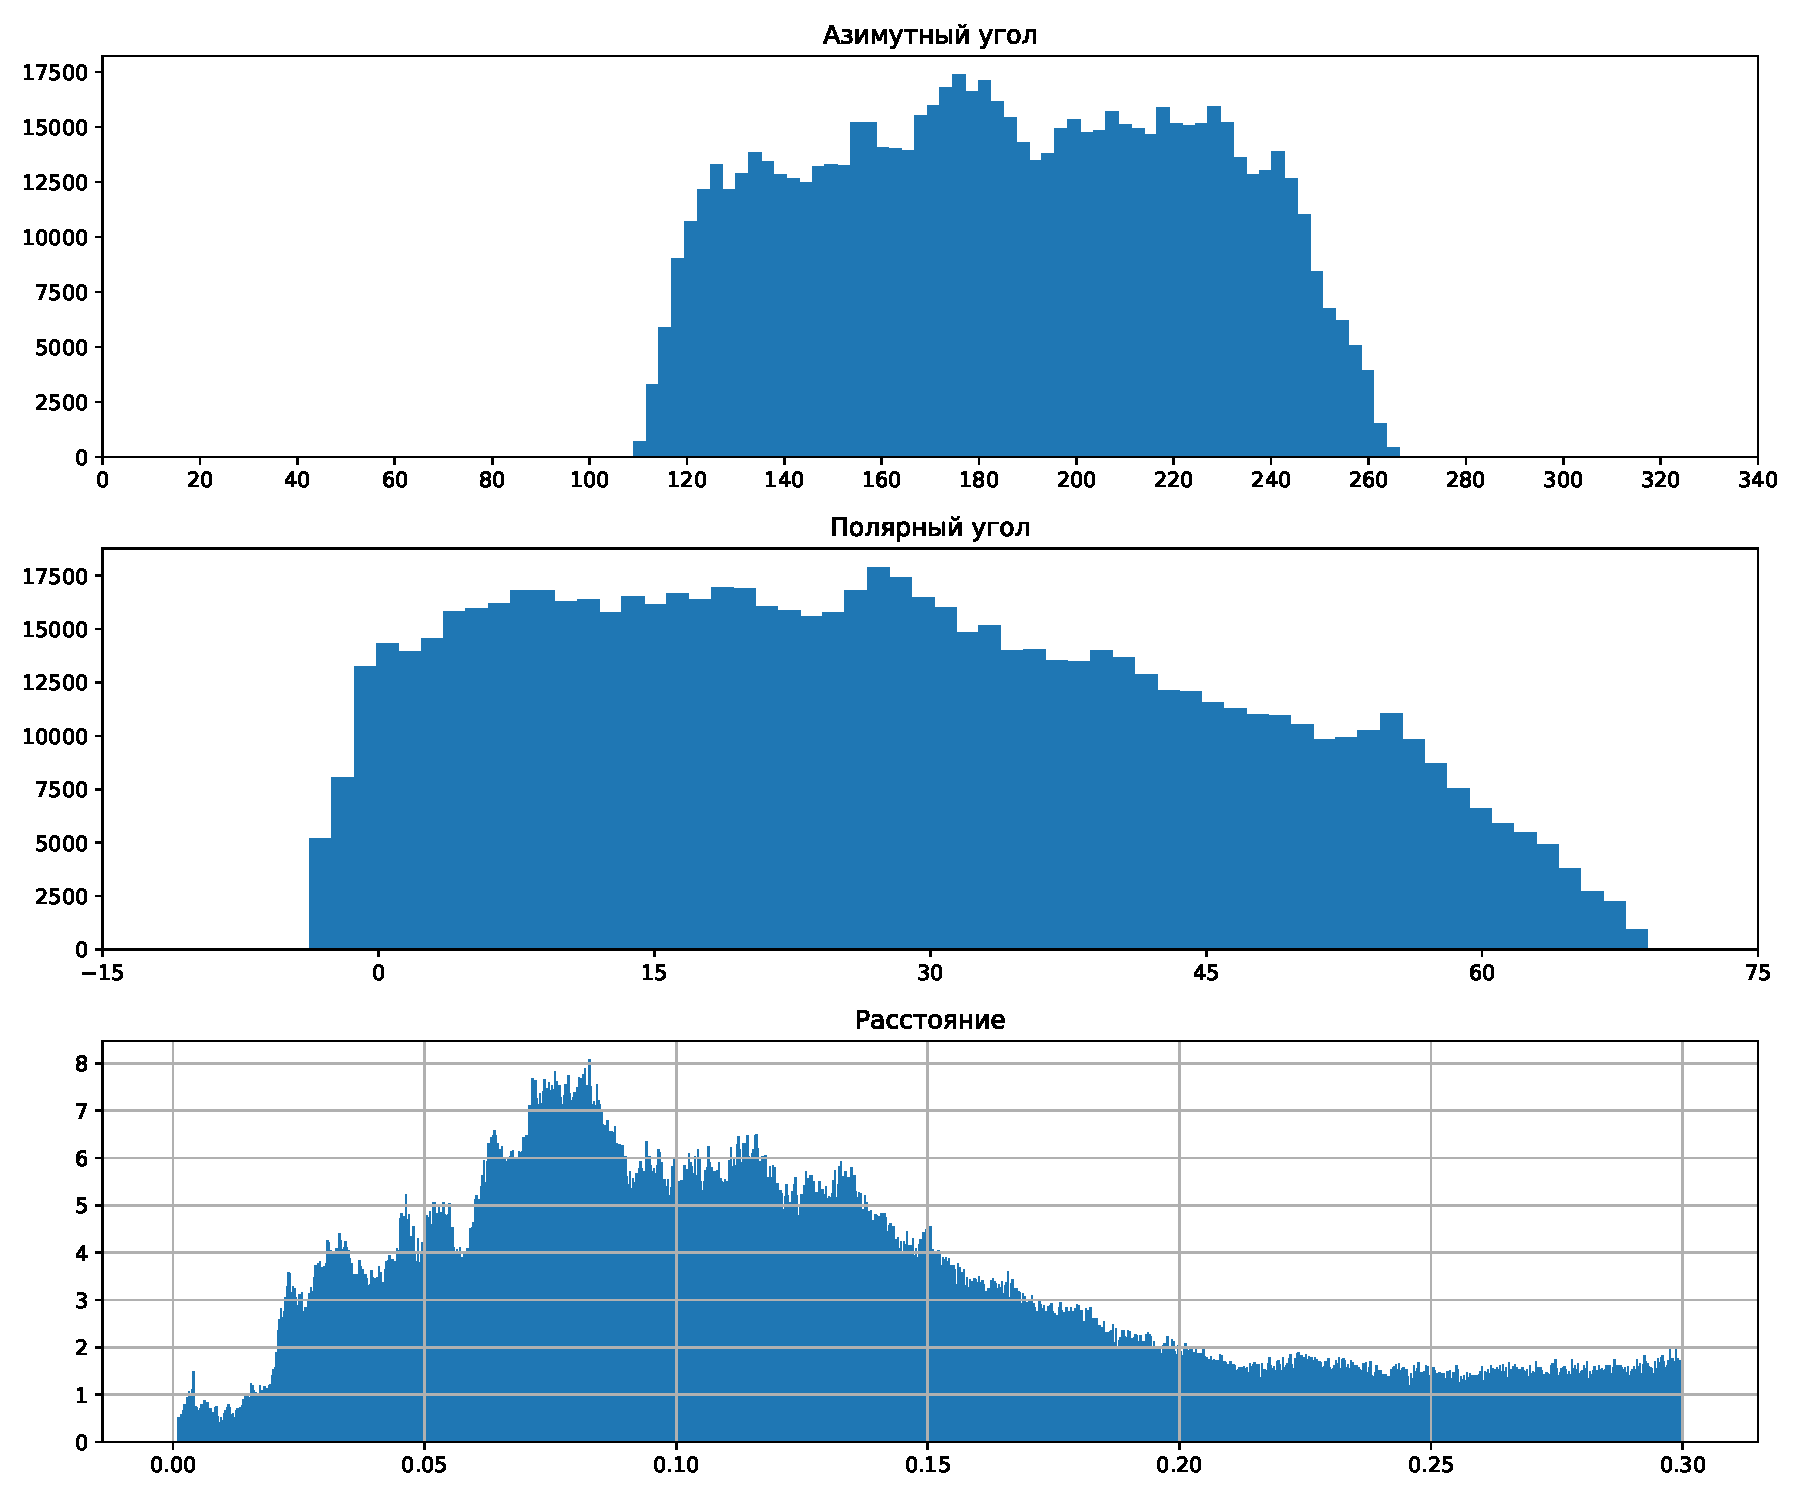
\includegraphics[width=12cm, height=13cm]{distrib.pdf}
  \caption{Распределение координат галактик}
  \label{distrib_coords}
\end{figure}



\begin{table}[h]
\begin{center}
\begin{tabular}{|l|llllllll|}
\hline

DBSCAN\_5   & 40329 & 25264 & 4665 & 4071 & 3550 & 815 & 583 & 561\\\hline
DBSCAN\_4   & 760 & 777 &  475 & 365 & 342 & 307 & 304 & 286 \\
\hline
\end{tabular}
\caption{Изменение функции потерь при дифференциальной эволюции}\label{loss_dif}
\end{center}
\end{table}



\begin{table}[h]
\begin{center}
\begin{tabular}{|l|llllllll|}
\hline
DBSCAN\_5   & 18620 & 18620 & 8365 & 6995 & 3517 & 3315 & 2977 & 2693\\
DBSCAN\_5 NH& 2218 & 1113 & 1047 & 1001 & 936 & 912 & 845 & 840\\ \hline
DBSCAN\_4   & 28683 & 18634 &  4989 & 2713 & 1535 & 1366 & 1270 & 1151\\
DBSCAN\_4 NH& 2021 & 937 & 835 & 663 & 662 & 662 & 667 & 604\\ \hline
DBSCAN\_1   & 117536 & 14698 &  3787 & 2587 & 1777 & 1691 & 1335 & 1201\\
DBSCAN\_1 NH& 3518 & 3067 & 1447 & 1335 & 1201 & 10850 & 982 & 972\\

\hline
\end{tabular}
\caption{Наибольшие по размеру кластеры}\label{hugest_clusters}
\end{center}
\end{table}

\newpage

\section{Заключение}

В данной работе был предложен подход, основанный на дифференциальной эволюции и алгоритме DBSCAN для решения залачи кластеризации сильно зашумленных данных с некоторой известной априорной информацией о распределении кластеров. Данный подход отличается от VDBSCAN тем, что не требует определения множества параметров eps с помощью графика распределений расстояний до k-го соседа (что очень трудно сделать в сильно зашумлённых данных).

Была решена задача кластеризации галактик по каталогу SDSS.
В дальнейшем с помощью варьирования или замены функций (\ref{F_num_clusters}, \ref{F_num_in1cluster}) на другие, выражающие иные априорные представления (характерный размер кластеров в единицах расстояния, их форма), возможно улучшить результаты этой кластеризации

\newpage


\section{Литература}

\begin{thebibliography}{2}

\bibitem{cluster_class}
M. Steinbach, V. Kumar, ''Cluster Analysis: Basic Concepts and Algorithms'', January 2005

\bibitem{VDBSCAN}
Peng Liu, Dong Zhou, Naijun Wu,  ''VDBSCAN: Varied Density Based Spatial Clustering of Applications with Noise'', 2007 International Conference on Service Systems and Service Management

\bibitem{AutoVDBSCAN}
A. Özekes, F. Ozge Ozkok et al, ''AutoVDBSCAN: An Automatic and Level-Wise Varied-Density Based Anomaly Detection Algorithm'',  2018
Conference: 7th International Conference on Advanced Technologies (ICAT'18)

\bibitem{BDE-DBSCAN}
A. Karami, R. Johansson, ''Choosing DBSCAN Parameters Automatically using
Differential Evolution'', 2014 International Journal of Computer Applications (0975 8887) Volume 91 - No.

\bibitem{dif_evol}
R. M. Storn, K. Price, ''Differential Evolution: A Simple and Efficient Adaptive Scheme for Global Optimization Over Continuous Spaces'', 1995 Journal of Global Optimization

\bibitem{SDSS}
SDSS Collaboration, ''The thirteen data release of the Sloan Digital Sky Server: first spectroscopic data from SDSS-IV survey mapping nearby galaxies at Apache point obdervatory'', 2017, arxiv.org

\bibitem{Abell}
Abell, G. O., ''The distribution of rich clusters of galaxies. A catalogue of 2712 rich clusters found on the National Geographic Society Palomar Observatory Sky Survey'', 1958, The Astrophysical Journal Supplement Series, 3,: 211—288.

\end{thebibliography}


\end{document} 